\section{INTERFEROMETRÍA}

\subsection{Introducción}
\begin{frame}{INTERFEROMETRÍA}
	\framesubtitle{Introducción}

	¿Qué ocurre cuando dos ondas del mismo tipo se encuentran?

	\url{https://www.youtube.com/watch?v=1PuzdU2RvW8}
	\url{https://www.youtube.com/watch?v=faAPLf7yPkl}

	%%%Imagen: http://www.principiamarsupia.com/wp-content/uploads/2016/02/pond.jpg
\end{frame}



\subsection{Interferencia Constructiva y Destructiva}

\begin{frame}{INTERFEROMETRÍA}
	\framesubtitle{Interferencia Constructiva y Destructiva}
	Para interferencia constructiva:
	\begin{equation}
		\Delta x = m \lambda , m=0, \pm 1, \pm 2...
	\end{equation}
	Para interferencia destructiva:
	\begin{equation}
		\Delta x = \frac{m\lambda}{2} , m=1, 3, 5...
	\end{equation}

  \begin{figure}
    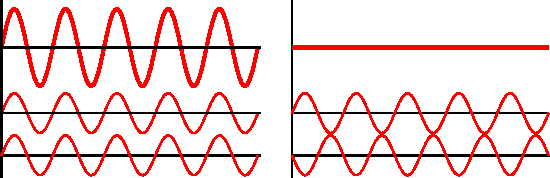
\includegraphics[scale=1]{juanse/interference.pdf}
    \caption{Interferencia entre ondas\footnotemark{}.}
  \end{figure}
  \vspace{-5mm}\footnotetext{\bibentry{interferencia}}
\end{frame}



\subsection{Inteferómetro de Michelson}
\begin{frame}{INTERFEROMETRÍA}
	\framesubtitle{Interferómetro de Michelson}
  \begin{figure}
    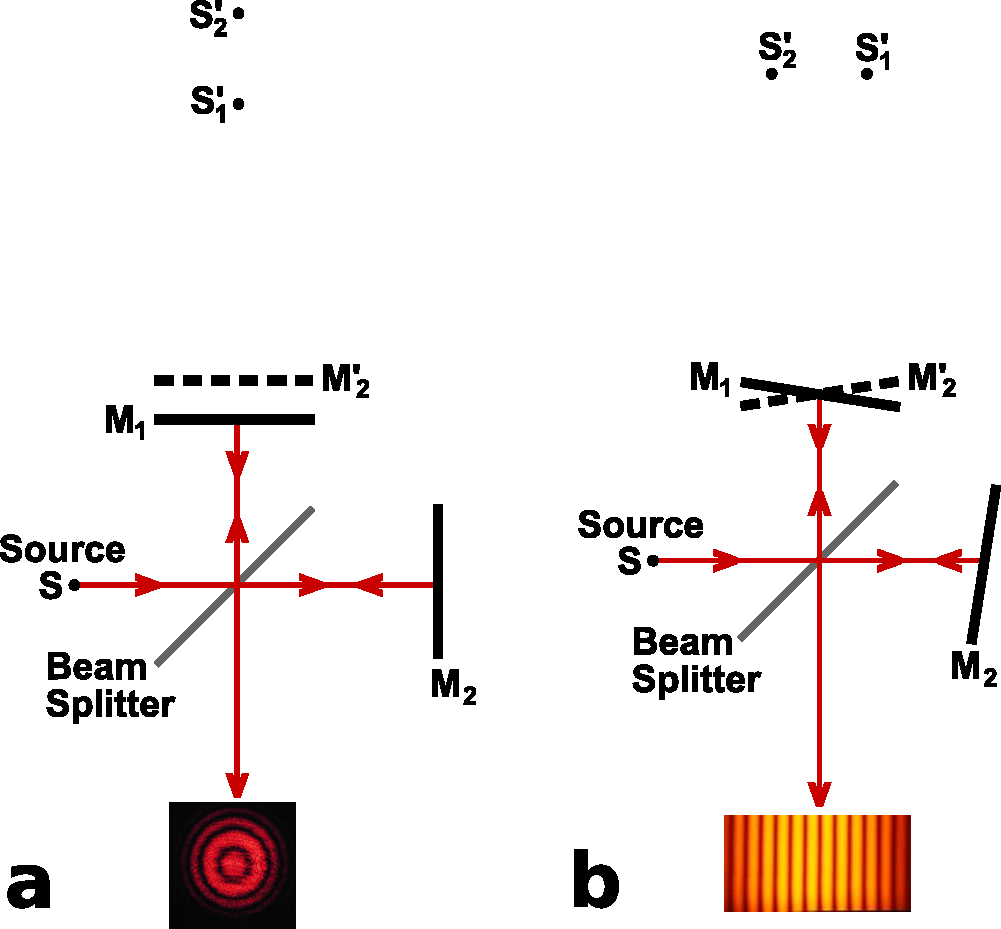
\includegraphics[scale=0.34]{juanse/michelson.pdf}
    \caption{Interferómetro de Michelson\footnotemark{}.}
  \end{figure}
  \vspace{-5mm}\footnotetext{\bibentry{michelson}}
\end{frame}




\subsection{Aplicaciones}

\begin{frame}{INTERFEROMETRÍA}
\framesubtitle{Aplicaciones}
\begin{multicols}{2}
	\textbf{Medición de Ondas Gravitacionales\\}
	Este interferómetro, en conjunto con cavidades de Fabry-Perot, permitió a LIGO medir la existencia de ondas gravitacionales
	en el 2015\footnote{\bibentry{ligo}}.
	\vfill\null

	\textbf{Experimento de Michelson-Morley\\}
	En 1920, Michelson y Morley intentaron demostrar la existencia del éter por medio de esta configuración. Sin embargo, no se logró demostrar su existencia.
\end{multicols}
\url{https://ligo.caltech.edu/system/video_items/files/21/Einsteins_messengers_hi_res_Nov_17_MPEG720p.mp4?1447873693}
\end{frame}

\begin{frame}{INTERFEROMETRÍA}
	\framesubtitle{Aplicaciones}
	\begin{multicols}{2}

	\textbf{Medir calidad de una superficie\\}

	La interferometría se puede utilizar para medir qué tan plana es una superficie, por medio de las franjas que éste presenta.

	\vfill\null

	\textbf{Interferómetro de Twyman-Green\\}
	Es una variación del interferómetro de Michelson para probar el funcionamiento de algun tipo de lente.
\end{multicols}
	\begin{figure}
		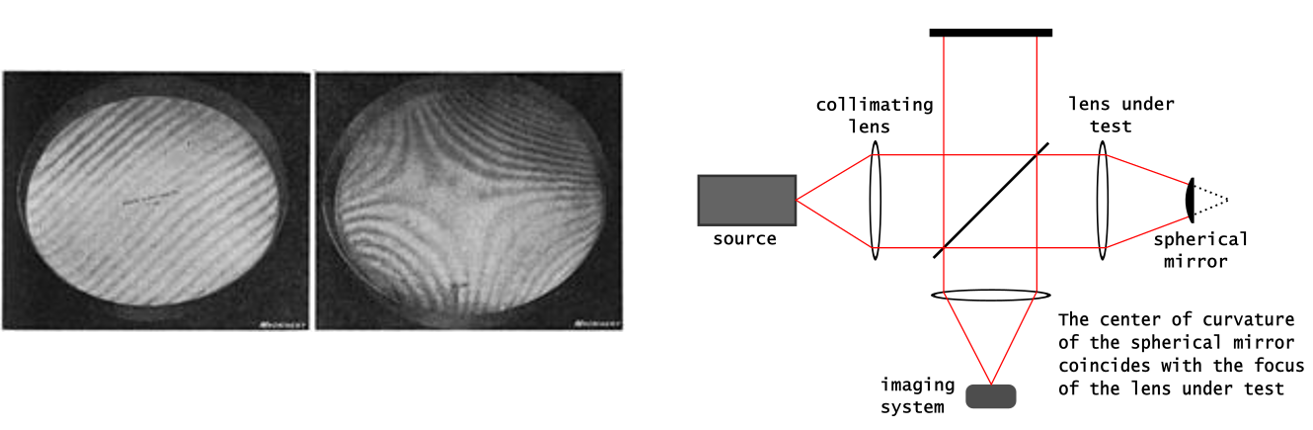
\includegraphics[scale=0.4]{juanse/twyy.png}
		\caption{Algunas aplicaciones de la interferometría\footnotemark{}\footnotemark{}.}
	\end{figure}
	\addtocounter{footnote}{-1}
	\footnotetext{\bibentry{fringes}}
	\addtocounter{footnote}{1}
	\footnotetext{\bibentry{twy}}
	\vspace{-1cm}
\end{frame}
